\documentclass[12pt]{beamer}
\usepackage{datetime}
\usepackage{animate}
\usetheme{Berlin}

\title[Employer Search and Screening in an Online Labor Market]{Employer Search and\\Screening in an Online\\Labor Market}
\author{John J. Horton}
\institute{oDesk Research}

\setbeamertemplate{footline}{%
  \begin{beamercolorbox}[sep=1mm,wd=\paperwidth,leftskip=1mm,rightskip=1mm]{footlinecolor}
    \hspace{1mm}%
    \tiny{\insertdate}
    \hfill
  \end{beamercolorbox}%
}

%gets rid of navigation symbols
\setbeamertemplate{navigation symbols}{}

\newcommand*\ouritem{%
\item[\color{black}\scalebox{0.9}{\textbullet}]}

\begin{document}

\setlength{\baselineskip}{12mm}
\fontsize{10mm}{12mm}\selectfont

\begin{frame}
\begin{center}
Employer Search and\\
Screening in an Online\\
Labor Market

\vspace{3mm}

\large
John J. Horton\\
oDesk Research
\end{center}
\end{frame}

\begin{frame}{}
\begin{center}
Matching markets have

search screening costs
\end{center}
\end{frame}

\begin{frame}{}
\Large
\begin{itemize}
\ouritem What \emph{are} my options?

\ouritem \emph{How good} is each option for me?
\end{itemize}
\end{frame}

\begin{frame}{}
\begin{animateinline}[autoplay]{2}
\begin{minipage}[c]{1\textwidth}
\begin{center}
\Large

\begin{figure}[H] \centering 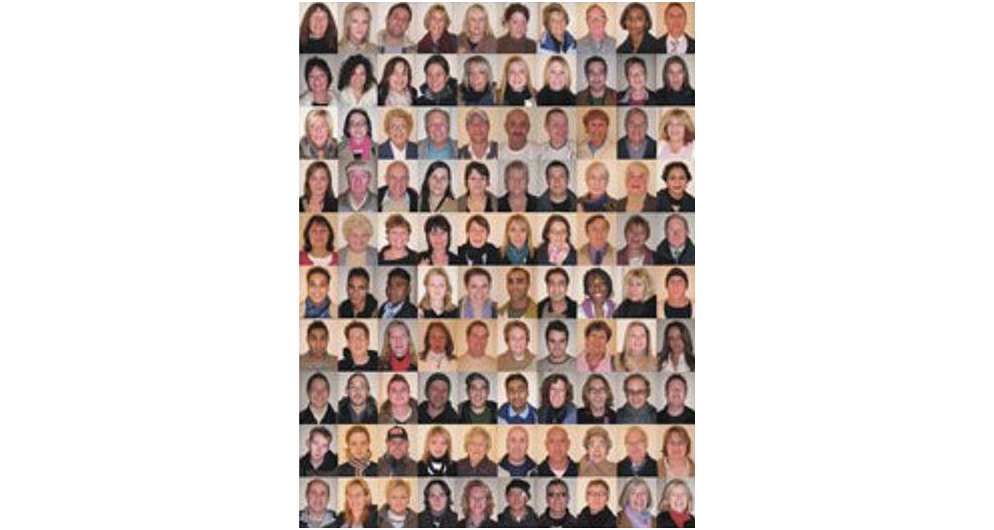
\includegraphics[width=100mm]{people_animation_1.png} \end{figure}

100 people
\end{center}
\end{minipage}
\end{animateinline}
\end{frame}

\begin{frame}{}
\begin{animateinline}[autoplay]{10}
\multiframe{11}{i=1+1}{
\begin{minipage}[c]{1\textwidth}
\begin{center}
\Large

\begin{figure}[H] \centering \includegraphics[width=100mm]{people_animation_\i.png} \end{figure}

100 people
\end{center}
\end{minipage}
}
\newframe
\multiframe{9}{i=11+1}{
\begin{minipage}[c]{1\textwidth}
\begin{center}
\Large

\begin{figure}[H] \centering \includegraphics[width=100mm]{people_animation_\i.png} \end{figure}

1,000 people
\end{center}
\end{minipage}
}
\end{animateinline}
\end{frame}

\begin{frame}{}
\begin{animateinline}[autoplay]{10}
\multiframe{5}{i=1+1}{
\begin{minipage}[c]{1\textwidth}
\begin{center}
\Large

\begin{figure}[H] \centering \includegraphics[width=100mm]{people_animation_2_\i.png} \end{figure}

1,000 people
\end{center}
\end{minipage}
}
\newframe
\multiframe{6}{i=6+1}{
\begin{minipage}[c]{1\textwidth}
\begin{center}
\Large

\begin{figure}[H] \centering \includegraphics[width=100mm]{people_animation_2_\i.png} \end{figure}

100,000 people
\end{center}
\end{minipage}
}
\end{animateinline}
\end{frame}

\end{document}